\def\year{2021}\relax
%File: formatting-instruction.tex
\documentclass[letterpaper]{article} % DO NOT CHANGE THIS
\usepackage{aaai20}  % DO NOT CHANGE THIS
\usepackage{times}  % DO NOT CHANGE THIS
\usepackage{helvet} % DO NOT CHANGE THIS
\usepackage{courier}  % DO NOT CHANGE THIS
\usepackage[hyphens]{url}  % DO NOT CHANGE THIS
\usepackage{graphicx} % DO NOT CHANGE THIS
\urlstyle{rm} % DO NOT CHANGE THIS
\def\UrlFont{\rm}  % DO NOT CHANGE THIS

\usepackage{amssymb,amsmath,bm}
\usepackage{graphics,adjustbox}
\usepackage{tikz}
\usepackage{subcaption}
\usepackage{siunitx}
\sisetup{unitsep = \cdot}

\usepackage[figuresright]{rotating}
\usepackage[colorinlistoftodos]{todonotes}
\usepackage[english,algo2e,algoruled,vlined,linesnumbered]{algorithm2e}   % package for algorithm
\usepackage{enumerate}

\usepackage{easyReview}
\newtheorem{assumption}{Assumption}


\DeclareMathOperator*{\argmin}{arg min}


\frenchspacing  % DO NOT CHANGE THIS
\setlength{\pdfpagewidth}{8.5in}  % DO NOT CHANGE THIS
\setlength{\pdfpageheight}{11in}  % DO NOT CHANGE THIS
%\nocopyright
%PDF Info Is REQUIRED.
% For /Author, add all authors within the parentheses, separated by commas. No accents or commands.
% For /Title, add Title in Mixed Case. No accents or commands. Retain the parentheses.
 \pdfinfo{
/Title (Smart Sanitizing Indoor Mobile Robot: Design and Development)
/Author (Brian Lauer, Nicoulas Shepard, Fazel Keshtkar, and Md Suruz Miah)
} %Leave this	
% /Title ()
% Put your actual complete title (no codes, scripts, shortcuts, or LaTeX commands) within the parentheses in mixed case
% Leave the space between \Title and the beginning parenthesis alone
% /Author ()
% Put your actual complete list of authors (no codes, scripts, shortcuts, or LaTeX commands) within the parentheses in mixed case. 
% Each author should be only by a comma. If the name contains accents, remove them. If there are any LaTeX commands, 
% remove them. 

% DISALLOWED PACKAGES
% \usepackage{authblk} -- This package is specifically forbidden
% \usepackage{balance} -- This package is specifically forbidden
% \usepackage{caption} -- This package is specifically forbidden
% \usepackage{color (if used in text)
% \usepackage{CJK} -- This package is specifically forbidden
% \usepackage{float} -- This package is specifically forbidden
% \usepackage{flushend} -- This package is specifically forbidden
% \usepackage{fontenc} -- This package is specifically forbidden
% \usepackage{fullpage} -- This package is specifically forbidden
% \usepackage{geometry} -- This package is specifically forbidden
% \usepackage{grffile} -- This package is specifically forbidden
% \usepackage{hyperref} -- This package is specifically forbidden
% \usepackage{navigator} -- This package is specifically forbidden
% (or any other package that embeds links such as navigator or hyperref)
% \indentfirst} -- This package is specifically forbidden
% \layout} -- This package is specifically forbidden
% \multicol} -- This package is specifically forbidden
% \nameref} -- This package is specifically forbidden
% \natbib} -- This package is specifically forbidden -- use the following workaround:
% \usepackage{savetrees} -- This package is specifically forbidden
% \usepackage{setspace} -- This package is specifically forbidden
% \usepackage{stfloats} -- This package is specifically forbidden
% \usepackage{tabu} -- This package is specifically forbidden
% \usepackage{titlesec} -- This package is specifically forbidden
% \usepackage{tocbibind} -- This package is specifically forbidden
% \usepackage{ulem} -- This package is specifically forbidden
% \usepackage{wrapfig} -- This package is specifically forbidden
% DISALLOWED COMMANDS
% \nocopyright -- Your paper will not be published if you use this command
% \addtolength -- This command may not be used
% \balance -- This command may not be used
% \baselinestretch -- Your paper will not be published if you use this command
% \clearpage -- No page breaks of any kind may be used for the final version of your paper
% \columnsep -- This command may not be used
% \newpage -- No page breaks of any kind may be used for the final version of your paper
% \pagebreak -- No page breaks of any kind may be used for the final version of your paperr
% \pagestyle -- This command may not be used
% \tiny -- This is not an acceptable font size.
% \vspace{- -- No negative value may be used in proximity of a caption, figure, table, section, subsection, subsubsection, or reference
% \vskip{- -- No negative value may be used to alter spacing above or below a caption, figure, table, section, subsection, subsubsection, or reference

\setcounter{secnumdepth}{0} %May be changed to 1 or 2 if section numbers are desired.

% The file aaai20.sty is the style file for AAAI Press 
% proceedings, working notes, and technical reports.
%
\setlength\titlebox{2.5in} % If your paper contains an overfull \vbox too high warning at the beginning of the document, use this
% command to correct it. You may not alter the value below 2.5 in
\title{Smart Sanitizing Indoor Mobile Robot: Design and Development}
%Your title must be in mixed case, not sentence case. 
% That means all verbs (including short verbs like be, is, using,and go), 
% nouns, adverbs, adjectives should be capitalized, including both words in hyphenated terms, while
% articles, conjunctions, and prepositions are lower case unless they
% directly follow a colon or long dash
\author{~%
Brian Lauer\textsuperscript{\rm 1}, Nicoulas Shepard\textsuperscript{\rm 1},
Fazel Keshtkar\textsuperscript{\rm 2}, and Md Suruz Miah\textsuperscript{\rm 1}
\\  
\textsuperscript{\rm 1}Electrical and Computer Engineering, Bradley University, Peoria, IL, USA; emails:~\{blauer,nshepard\}@mail.bradley.edu,~smiah@bradley.edu\\
\textsuperscript{\rm 2}Computer Science, Math. and Science, St John's University, Queens, NY, USA; email:~keshtkaf@stjohns.edu
}
 \begin{document}

\maketitle

\begin{abstract}
\end{abstract}

\section{Introduction}
\label{sec:introduction}

\section{Existing Sanitizing Robots} 
\label{sec:Literature}




\section{System Architecture}
\label{sec:SystemArchitecture}

\todo[inline]{Discuss two different architecture that we propose}

\begin{figure}[htpb]
  \centering
  \begin{subfigure}[b]{0.5\textwidth}
    \centering
    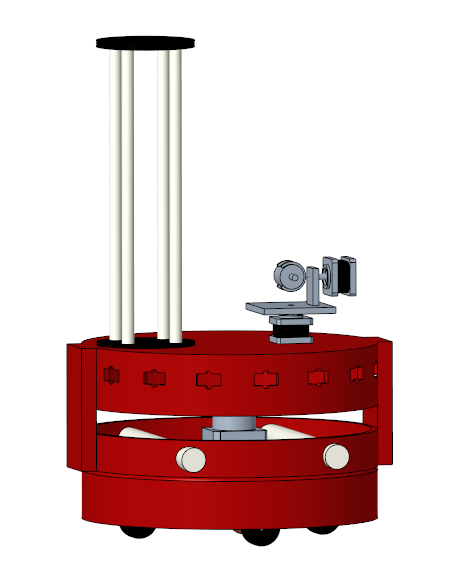
\includegraphics[scale=0.25]{../figs/img/frontViewScreenshotB}
    \caption{Overall design of the proposed smart sanitizing robot.}
    \label{fig:frontViewScreenshotB}
  \end{subfigure}
  \begin{subfigure}[b]{.5\textwidth}
    \centering
    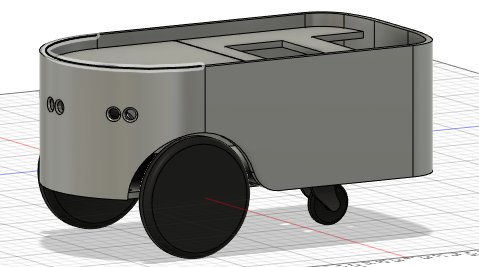
\includegraphics[scale=0.1]{../figs/img/v2BodyDesign}
    \caption{Body design}
  \end{subfigure}
  \begin{subfigure}[b]{.5\textwidth}
    \centering
    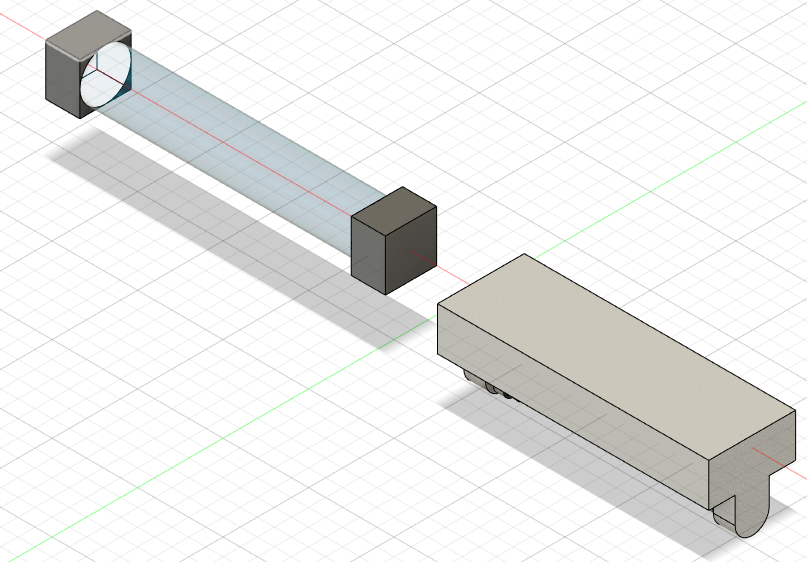
\includegraphics[scale=0.1]{../figs/img/v2UVLamp}
    \subcaption{UV lamp model}
  \end{subfigure}
  \begin{subfigure}[b]{.5\textwidth}
    \centering
    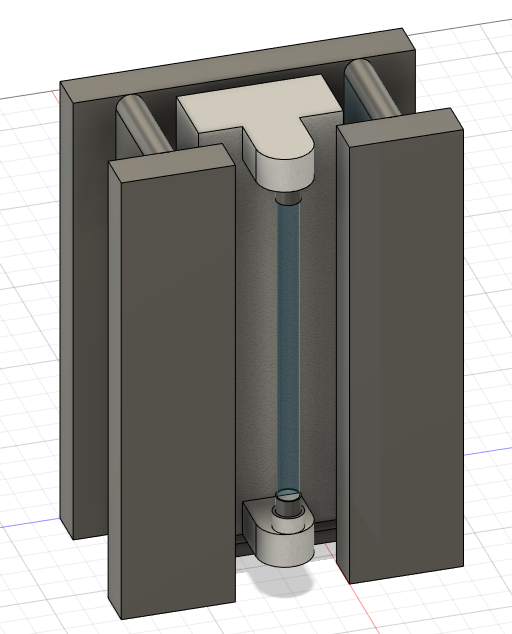
\includegraphics[scale=0.1]{../figs/img/v2UVLampConveyor}
    \subcaption{UV lamp conveyor}
  \end{subfigure}
  \begin{subfigure}[b]{.5\textwidth}
    \centering
    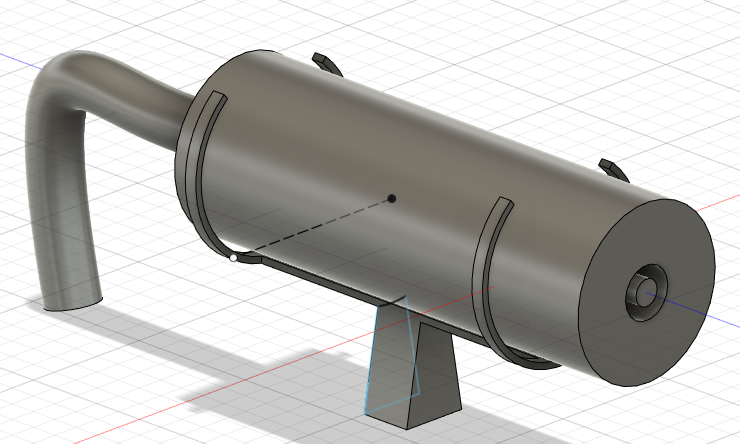
\includegraphics[scale=0.1]{../figs/img/v2SprayerMount}
    \subcaption{Disinfectant sprayer mount}
  \end{subfigure}
  \caption{Design of Proposed Sanitizing Robots.}
  \label{fig:ArchitecturesOfSanitizingRobot}
\end{figure}


\subsection{Features}
\label{sec:Features}

\subsection{Operating Principle}
\label{sec:OperatingPrinciple}



\section{Detailed Design}
\label{sec:DetailedDesign}



\section{Real-Time Computer Experiment}
\label{sec:RealTimeComputerExperiment}


\section{Conclusion} \label{sec:conclusion}


% \bibliographystyle{aaai}
% \bibliography{bib/refsSuruzWeb,bib/refsMultiAgent,bib/refsRoboticsJournals,bib/refsRoboticsConferences,bib/refsGenericControl,bib/refsBooksTRTheses,bib/refsReinforcementLearningADP,bib/refsRL-Keshtkar}

\end{document}

%%% Local Variables:
%%% mode: latex
%%% TeX-master: t
%%% End:
